\section{Results and Analysis}
\subsection{RQ1: Structural Fault Rejection}
Table~\ref{tab:results} reports the three pipeline conditions using the same labeled corpus. The full contract classifies all 72 instances correctly in each process, whereas schema-only validation classifies 40 correctly and schema plus topology classifies 56 correctly. This corresponds to accuracies of $100.00\%$, $55.56\%$, and $77.78\%$, respectively, with zero sample standard deviation for classification across runs. These are conformance results on constructed instances. They are not estimates of AI generation accuracy, production failure probability, or correctness over arbitrary infrastructure.
\begin{table}[t]
\caption{Three-process results. Values with uncertainty show mean $\pm$ sample SD; timing includes cloning. Bold denotes the highest structural accuracy on this corpus.}
\label{tab:results}
\centering\footnotesize
\begin{tabular}{lrrrr}
\toprule
Pipeline & Accuracy (\%) & False accepts / 48 & False rejects / 24 & Time ($\mu$s) \\
\midrule
Schema only & $55.56 \pm 0.00$ & $32 \pm 0$ & 0 & $41.3 \pm 8.9$ \\
Schema + topology & $77.78 \pm 0.00$ & $16 \pm 0$ & 0 & $57.6 \pm 26.0$ \\
Full contract & $\mathbf{100.00 \pm 0.00}$ & $0 \pm 0$ & 0 & $72.9 \pm 14.1$ \\
\bottomrule
\end{tabular}

\end{table}
Schema-only validation rejects the 16 shape/type faults but accepts all 32 invalid topology or reference instances. Its false-acceptance rate among invalid cases is therefore $66.67\%$. Adding topology checks rejects another 16 cases and reduces that rate to $33.33\%$. The complete contract rejects the remaining reference faults and has no structural false accepts in this corpus. Every condition accepts all 24 labeled valid cases, so the observed gain does not trade away any of the corpus's supported positives. This does not establish the absence of false rejections on other valid architectures or configuration combinations.

Fig.~\ref{fig:errors} breaks the errors down by fault class. The pattern follows the constraints removed by the ablations: document-shape rules cannot detect duplicate graph identifiers or unsupported relationships, while topology checks alone cannot inspect configuration strings for unbound references. Each bar summarizes 16 constructed cases, and the same counts occur in every process. The result supports retaining all three layers in the application's acceptance boundary. It does not demonstrate that the selected fault classes occur with the same frequency in real AI responses or user-created sketches.
\begin{figure}[t]
\centering
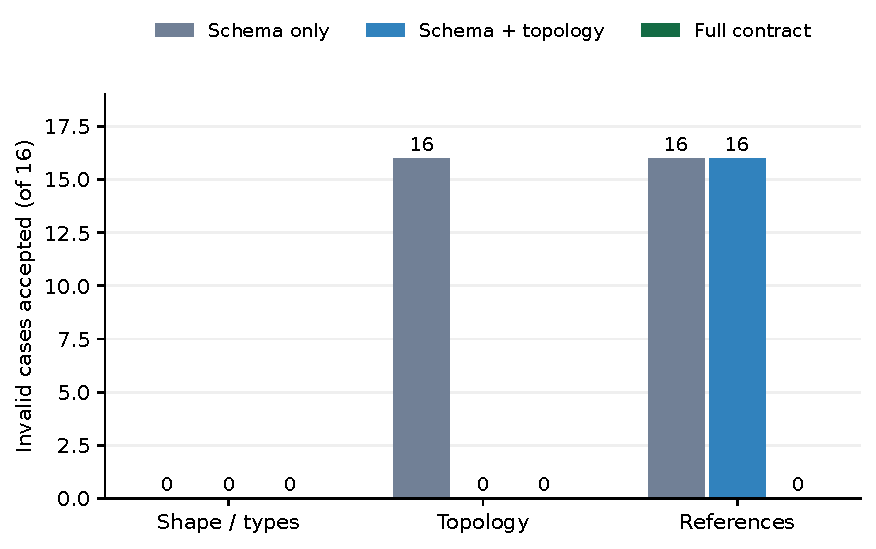
\includegraphics[width=.95\linewidth]{validation-errors.pdf}
\caption{Invalid instances accepted by fault category and validation pipeline. Each category contains 16 cases; counts are identical across the three processes.}
\label{fig:errors}
\end{figure}
The ablation is particularly informative for configuration references. The middle pipeline still verifies that a graph has compatible, known endpoints and an execution ordering, yet it accepts references without the required source binding. Thus an accepted topology is insufficient to connect configuration values to that topology. Conversely, a schema-valid string that resembles an output expression has no operational meaning until the source relationship and later output availability are checked. The improvement measured here is fault detection added by these particular layers, not a new property of topological sorting or schema validation.


The corpus makes the effect of each layer countable. Relative to schema alone, adding topology checks changes the decisions on 16 of the 72 instances, raising accuracy by 22.22 percentage points. Reference analysis changes a different 16 decisions by the same amount. The pipeline retains the shape filter throughout, so the gains are additive for these assigned categories. That arithmetic depends on equal category sizes and the construction of single dominant faults. In an observed mixture of defects, errors could overlap and the gains would depend on which defects occur most often. For instance, a missing source node may cause a graph error before a later configuration reference is even examined. The experiment describes the final rejection decision and does not measure the completeness of the diagnostic messages.

Acceptance of the valid fixtures also needs qualification. A positive fixture for a service demonstrates at least one admitted configuration pattern. It does not test every combination of optional parameters, every account setting, or every interaction among supported services. The recorded corpus and case-level decisions allow a reader to identify exactly which patterns were exercised. A suite drawn from naturally occurring authoring errors would provide complementary evidence about which checks matter most in everyday use.

\subsection{RQ2: Processing Cost and Boundary Behavior}
The measured clone-plus-validation means are $41.3\pm8.9$ microseconds for schema only, $57.6\pm26.0$ microseconds for schema plus topology, and $72.9\pm14.1$ microseconds for the full contract. Fig.~\ref{fig:latency} presents these per-process statistics with error bars. The complete pipeline performs additional graph traversal, reference scanning, and exception handling, which explains the direction of the mean differences. The substantial variability and only three processes do not support a statistical claim about the exact marginal cost or a universal performance ranking. All measurements concern small fixtures after warm-up, with no network communication.
\begin{figure}[t]
\centering
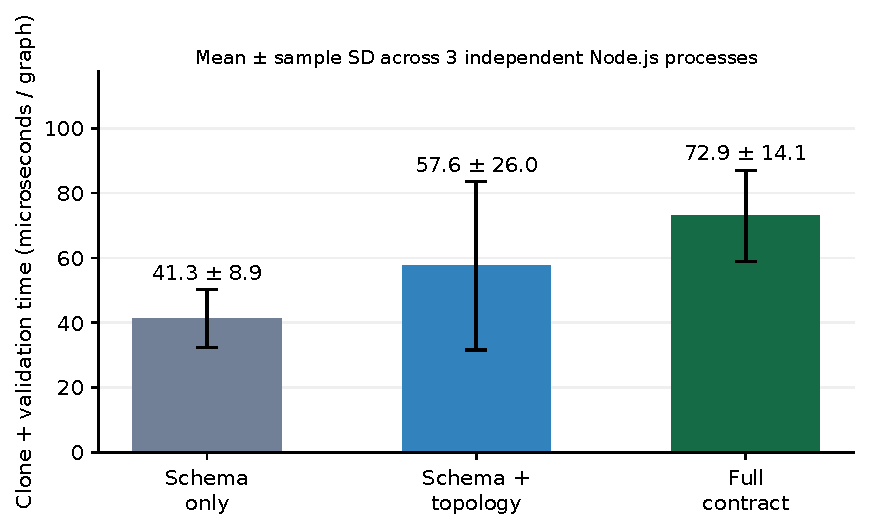
\includegraphics[width=.95\linewidth]{validation-latency.pdf}
\caption{Mean local validation cost and sample SD across three fresh processes. Error bars describe process-level variability, not uncertainty in cloud-deployment latency.}
\label{fig:latency}
\end{figure}
Table~\ref{tab:boundary} records six controls that the full graph contract accepts in each process. They deliberately probe distinctions outside the structural labels: output-field existence, deployment completeness, additional publish restrictions, execution-role trust, identifier availability, and external user requirements. Their acceptance is not hidden inside the structural accuracy score. Instead, it explains why that score cannot be used as a global safety percentage.
\begin{table}[t]
\caption{Accepted boundary controls and the check still needed. All six pass graph validation; none was deployed.}
\label{tab:boundary}
\centering\small
\begin{tabularx}{\linewidth}{lX}
\toprule
Control & Interpretation / additional check \\
\midrule
Unknown output field & Direct source exists; runtime output resolution must check the field. \\
Incomplete Lambda draft & Draft schema permits missing execution fields; publish must reject incompleteness. \\
Public S3 / CloudFront origin & Graph shape permits the setting; publish preflight rejects the combination. \\
Wrong IAM trusted service & Type-compatible attachment alone does not prove execution-role suitability. \\
Unverified AMI literal & A string does not prove an identifier exists in the selected region. \\
Unmet SNS requirement & A valid S3 graph does not satisfy an independent request for SNS. \\
\bottomrule
\end{tabularx}
\end{table}
The six controls are explanatory examples, not a measured distribution of operational defects. Several require information intentionally unavailable to the offline validator, while others belong to later application checks or a missing intent/policy oracle. No AWS deployment failure was observed here because no AWS operation was attempted. Together, the controls and ablations answer RQ2: the additional local checks have a measurable processing cost and a clearly limited acceptance meaning. A downstream study should evaluate publish preconditions, provider execution, intent satisfaction, and cleanup with separate denominators rather than extending the present $100\%$ conformance result to those outcomes.


The timing means should be interpreted alongside this decision analysis. The difference between the schema-only and full-contract means is 31.6 microseconds per graph in the recorded runs. The timer includes creating a fresh input and catching rejection exceptions, so both the work performed and the proportion of inputs that throw can influence it. It would be premature to assign the entire difference to reference traversal or extrapolate it to a user-facing response time. A dedicated scaling experiment would vary graph size and configuration depth while holding the acceptance mix constant, then report preparation, validation, and diagnostic costs separately.
